% Copyright (C) 2004-2006 Jed Brown and Ed Bueler
%
% This file is part of Pism.
%
% Pism is free software; you can redistribute it and/or modify it under the
% terms of the GNU General Public License as published by the Free Software
% Foundation; either version 2 of the License, or (at your option) any later
% version.
%
% Pism is distributed in the hope that it will be useful, but WITHOUT ANY
% WARRANTY; without even the implied warranty of MERCHANTABILITY or FITNESS
% FOR A PARTICULAR PURPOSE.  See the GNU General Public License for more
% details.
%
% You should have received a copy of the GNU General Public License
% along with Pism; if not, write to the Free Software
% Foundation, Inc., 51 Franklin St, Fifth Floor, Boston, MA  02110-1301  USA

\documentclass[11pt,final]{amsart}
\addtolength\topmargin{-.1in}
\addtolength\textheight{0.3in}
\addtolength{\oddsidemargin}{-.5in}
\addtolength{\evensidemargin}{-.5in}
\addtolength{\textwidth}{1.0in}
\newcommand{\normalspacing}{\renewcommand{\baselinestretch}{1.1}\tiny\normalsize}
\newcommand{\tablespacing}{\renewcommand{\baselinestretch}{1.0}\tiny\normalsize}
\normalspacing

\usepackage{bm,url,xspace,verbatim}

\ifx\pdftexversion\undefined
  \usepackage[final,dvips]{graphicx}
\else
  \usepackage[final,pdftex]{graphicx}
\fi

\renewcommand{\t}[1]{\texttt{#1}}
\newcommand{\Matlab}{\textsc{Matlab}\xspace}
\newcommand{\bU}{\mathbf{U}}
\newcommand{\eps}{\epsilon}

% note \beginV and \Vend are a pair, but they must be used as follows:
%   \beginV
%      ... stuff
%   \end{verbatim}
%   \Vend
% that is, "\end{verbatim}" still has to appear on a line by itself with no leading spaces
%\newcommand{\Vend}{ \rule{4.6in}{0.1mm}\end{quote} }
%\newcommand{\beginV}{ \begin{quote}\rule{4.6in}{0.1mm}\begin{verbatim} }
\newcommand{\Vend}{ \rule{4.6in}{0.1mm}\end{quote}\normalsize }
%\newcommand{\beginV}{ \small\begin{quote}\rule{4.6in}{0.1mm}\begin{verbatim} }
\newcommand{\beginV}{ \scriptsize\begin{quote}\rule{4.6in}{0.1mm}\begin{verbatim} }

\newcommand{\Vfile}[1]{ \begin{quote}\rule{4.6in}{0.1mm} \verbatiminput{#1} \rule{4.6in}{0.1mm}\end{quote} }


\title[PISM User's Manual]{PISM, a \underline{P}arallel \underline{I}ce \underline{S}heet \underline{M}odel: \\ User's Manual}

\author{Jed Brown and Ed $\text{Bueler}^\ast$}

\date{\today.  $\phantom{|}^\ast$\texttt{ffelb\@@uaf.edu}.  Manual version based on PISM revision 90.  Get PISM by Subversion: \texttt{svn co http://svn.gna.org/svn/pism/trunk pism}; update to latest version by \texttt{svn update}.} 

\begin{document}
\maketitle
\thispagestyle{empty}
%\tablespacing

\setcounter{tocdepth}{1}
\tableofcontents

\newpage
\phantom{bob}
\vspace{2in}
\begin{quote}
\textsl{Copyright (C) 2004--2007 Jed Brown and Ed Bueler}
\medskip

\noindent \textsl{This file is part of PISM.}
\medskip

\noindent \textsl{PISM is free software; you can redistribute it and/or modify it under the terms of the GNU General Public License as published by the Free Software Foundation; either version 2 of the License, or (at your option) any later version.}
\medskip

\noindent \textsl{PISM is distributed in the hope that it will be useful, but WITHOUT ANY WARRANTY; without even the implied warranty of MERCHANTABILITY or FITNESS FOR A PARTICULAR PURPOSE.  See the GNU General Public License for more details.}
\medskip

\noindent \textsl{You should have received a copy of the GNU General Public License along with PISM; see \emph{\texttt{pism/COPYING}}; if not, write to the Free Software Foundation, Inc., 51 Franklin St, Fifth Floor, Boston, MA  02110-1301 USA}
\end{quote}
\vspace{1in}
\normalspacing

\newpage
\section{Installation}

\renewcommand{\labelenumi}{\arabic{enumi}.~}
\begin{enumerate}
\item You will need a UNIX system with X Windows and internet access.  A GNU/Linux environment will be easiest but other UNIX versions have been used successfully.
\item You will need Subversion (\url{http://subversion.tigris.org/}) installed; it is automatic in current Linux distributions.
\item You will need MPI (= Message Passing Interface; \url{http://www-unix.mcs.anl.gov/mpi/}).  It would be reasonable to learn enough about MPI to know how to run a very simple C code on multiple processors using MPI.  There are multiple flavors of MPI, but choose one which works with PETSc, next.
\item Get PETSc = Portable Extensible Toolkit for Scientific computation from \url{http://www-unix.mcs.anl.gov/petsc/petsc-2/index.html}.
See the installation page for PETSc.  The ``lite'' form is fine if you are willing to depend on an internet connection for PETSc documentation.  Note that you will define environment variables \verb|PETSC_DIR| and \verb|PETSC_ARCH|.  When you run the configure script add the following options (note PISM uses shared libraries by default):

\verb|$ ./config/configure.py --with-shared|

\noindent Configuring and building Petsc takes a while.  After it finishes, ``\verb|make test|'' and watch the
result; Xwindows must be functional to see all tests.  If PETSc is already defined system-wide then it will be desirable to have a \verb|PETSC_ARCH| with the configuration above.  Note that the configuration of PETSc for a batch system requires special procedures described at the PETSc documentation site.
\item PISM uses NetCDF (\url{http://www.unidata.ucar.edu/software/netcdf/}) for a file format so you will need it installed in a location where the compiler/linker can find it, i.e.~on your \verb|PATH|.
\item PISM uses the FFTW and GSL libraries for to approximate the solid earth (bed) deformation under ice loads \cite{BLKfastearth}.  Therefore:
\renewcommand{\labelenumii}{(\roman{enumii})}\begin{enumerate}
\item If FFTW (\url{http://www.fftw.org/}) is installed and in a good system-wide place, do nothing.  Otherwise turn off PISM's attempt to build with it by setting the environment variable \verb|WITH_FFTW=0|.  PISM will work except for the bed deformation model described in the paper \cite{BLKfastearth}.
\item If GSL (\url{http://www.gnu.org/software/gsl/}) is installed and in a good system-wide place, do nothing.  Otherwise turn off PISM's attempt to build with it by setting the environment variable \verb|WITH_GSL=0|.  PISM will work except for the bed deformation model described in the paper above.\end{enumerate}

See Table \ref{tab:PISMdepends} for a summary of the dependencies on external libraries, as described so far.

\item \label{getPISMstep} Get the source for PISM by

\verb|svn co http://svn.gna.org/svn/pism/trunk pism|

\noindent A directory called ``\verb|pism/|'' will be created.  Note that if you are in that directory then ``\verb|svn update|'' will get the latest revision of PISM.
\item Enter directory \verb|pism/| and type ``\verb|make|''.  (\emph{PLEASE} report any problems you meet at this stage by sending us the output: \verb|ffelb@uaf.edu|.)  Several executables, including \verb|pismv|, \verb|pisms|, and \verb|pismr| should appear in the \verb|pism/obj/| subdirectory.
\item Try a serial verification run of PISM:

\verb|$  obj/pismv -test G -y 100|

\noindent If you see some output and a final 

\verb|writing model state to file 'verify.pb' ... done|

\noindent then PISM is working!  Note that at the end of this run you will get measurements of how close the numerical result is to the exact solution, that is, this is a verification run \cite{BBL}.
\item Try the MPI four processor version of the above run:

\verb|$  mpiexec -n 4 obj/pismv -test G -y 100|

\noindent This should work even if the is only one actual processor on your machine; MPI should run multiple processes on that processor.  The results should be the same---in particular the reported errors should be very nearly the same---but the results should appear faster if there really are four processors!
\item Try a verification run on a reasonably fine grid while watching the output under Xwindows:

\verb|$  obj/pismv -test G -Mx 101 -My 101 -Mz 101 -y 2000 -d HTc|
\item Running a verification test of the ice stream code looks like this:

\verb|$  obj/pismv -test I -Mx 5 -My 401 -verbose|

\noindent This will compare the numerical result to the exact solution appearing in \cite{SchoofStream}.
\item Running a 10,000 year (shortened) EISMINT II experiment F \cite{EISMINT00}) is this:

\verb|$  obj/pisms -eisII F -Mx 61 -My 61 -Mz 101 -y 10000|

\noindent Note that all of these runs, when completed, save the model state and can be restarted and continued.
\item Run a basic suite of verifications:

\verb|$  test/verifynow.sh|

\noindent The script is the serial version; we can send a multiprocessor version or you can modify it to be so.  If serial, this will take 2 to 6 hours.  Save the (one page or so of) output and send it to us if you want.
\end{enumerate}

\begin{table}
\caption{External library dependencies for PISM.}\label{tab:PISMdepends}
\begin{tabular}{@{}llll}\hline
\small
\textbf{Library} & \textbf{Site} & \textbf{Required?} & \textbf{Comment} \\ \hline
FFTW & \url{www.fftw.org} & \emph{no} & if not present  \\
 & & & \quad set \verb|WITH_FFTW=0| \\
GSL & \url{www.gnu.org/software/gsl} & \emph{no} &  if not present \\
 & & & \quad set \verb|WITH_GSL=0| \\
MPI & \url{www-unix.mcs.anl.gov/mpi} & \emph{required} & \\
NetCDF & \url{www.unidata.ucar.edu/software/netcdf} & \emph{required} & \\
PETSc & \url{www-unix.mcs.anl.gov/petsc/petsc-2/index.html} & \emph{required} & \\
Subversion & \url{subversion.tigris.org} & \emph{required} & \\
\hline
\normalsize
\end{tabular}
\end{table}

Have fun!  Please write to us anytime (\verb|ffelb@uaf.edu|).

Setting up PISM to model real ice sheets requires techniques not covered here, but that is something we welcome questions about and will seek to help with.

A final reminder with respect to installation:  Once you have checked out a copy of PISM using Subversion, as in step \ref{getPISMstep} above, you can update it to the latest version by \verb|svn update| in the \verb|pism/| directory.  Then you will want to \verb|make| again.


\clearpage
\newpage
\section{Getting started}

\subsection{Running the EISMINT II tests}  PISM's purpose is the realistic simulation of ice sheets.  But real ice sheet simulations require real data.  And real data is something we can't yet distribute under the GNU Public License.

So we describe how PISM does experiment F in the EISMINT II intercomparison \cite{EISMINT00}, in which one tries to approximate an unstable equilibrium and one gets the infamous ``spokes'' \cite{BBL}.  The prescribed grid has a grid with 60 subintervals in each direction of length 25km, but the vertical grid is not prescribed.  Runs are for 200,000 model years.

PISM knows about the conditions of the EISMINT II tests but PISM always allows choice of the grid in three dimensions.  PISM requires choice of the number of grid points in each direction to start.  We choose the standard 25km grid in the horizontal and use a 25 m (equally-spaced) grid in the vertical.  The executable is ``\t{pisms}'', with trailing ``\t{s}'' for the ``simplifed geometry mode'' of PISM.  Here is a short 2000 year run.

\beginV
user@host:~/pism$ obj/pisms -eisII F -Mx 61 -My 61 -Mz 201 -y 2000
PISMS (simplified geometry mode)
  [using flow law 0 (where 0=Paterson-Budd,1=cold P-B,2=warm P-B,3=Hooke,4=Goldsby-Kohlstedt)]
initializing EISMINT II experiment F ...
  [computational box for ice: ( 1500.00 km) x ( 1500.00 km) x ( 5000.00 m)]
  [grid cell dimensions     : (   25.00 km) x (   25.00 km) x (   25.00 m)]
running EISMINT II experiment F ...
$$$$$      YEAR (+    STEP[N$]):     VOL    AREA    MELTF     THICK0     TEMP0
$$$$$      0.00 (+  0.0000[0 ]):   0.000   0.000    0.000      0.000   223.150
$v$tf     60.00 (+ 60.0000[0m]):   0.017   0.628    0.000     30.000   223.150
$v$tf    120.00 (+ 60.0000[0m]):   0.034   0.628    0.000     60.000   223.538
$v$tf    180.00 (+ 60.0000[0m]):   0.051   0.628    0.000     90.000   223.869
$v$tf    240.00 (+ 60.0000[0m]):   0.068   0.628    0.000    120.000   224.162
$v$tf    300.00 (+ 60.0000[0m]):   0.085   0.631    0.000    150.000   224.425
$v$tf    360.00 (+ 60.0000[0m]):   0.102   0.631    0.000    180.000   224.667
$v$tf    420.00 (+ 60.0000[0m]):   0.119   0.631    0.000    210.000   224.898
$v$tf    480.00 (+ 60.0000[0m]):   0.136   0.631    0.000    240.000   225.117
\dots
$v$tf   1920.00 (+ 60.0000[0m]):   0.545   0.631    0.000    960.000   228.389
$v$tf   1980.00 (+ 60.0000[0m]):   0.562   0.631    0.000    990.000   228.487
$v$tf   2000.00 (+ 20.0000[0e]):   0.568   0.631    0.000   1000.000   228.520
done with run ... writing model state to file `simp_exper.pb' ... done.
\end{verbatim}
\Vend

This should have taken less than 30 seconds on any modern computer.  In a moment we will address the standard output information provided by PISM, shown above.

For now illustrate how to restart, complete, and save the 200,000 year run.  Note that the model state was stored in a file with a default name ``\texttt{simp\underline{ }exper.pb}''.  Let's give it a more useful name with

\verb|mv simp_exper.pb eisIIF2k.pb|

\noindent We will see in a moment an example of telling PISM how to name the output file, and how to choose its format.

The above was a single processor run, but let's suppose we have a four processor machine.  (Note that the following should work as stated on a single processor machine under most MPI installations.)  Let's run things in the background so we can continue to experiment.

\beginV
user@host:~/pism$ mpiexec -n 4 obj/pisms -eisII F -if eisIIF2k.pb -y 198000\
  -o eisIIF200k >> eisIIF.out &
[4] 7405
\end{verbatim}
\Vend

One can view the standard output by ``\t{less eisIIF.out}'' as it is running in the background.  Also ``\t{top}'' is a convenient tool to see the processor usage during the run.

While the above is running in the background, let's actually look at a few time steps by starting from the saved 2000 year state, using PISM's ``diagnostic viewers'':

\beginV
user@host:~/pism$ obj/pisms -eisII F -if eisIIF2k.pb -y 200 -d HTt
PISMS (simplified geometry mode)
  [using flow law 0 (where 0=Paterson-Budd,1=cold P-B,2=warm P-B,3=Hooke,4=Goldsby-Kohlstedt)]
initializing from PETSc binary format file  eisIIF2k.pb  ...
  [computational box for ice: ( 1500.00 km) x ( 1500.00 km) x ( 5000.00 m)]
  [grid cell dimensions     : (   25.00 km) x (   25.00 km) x (   25.00 m)]
running EISMINT II experiment F ...
$$$$$      YEAR (+    STEP[N$]):     VOL    AREA    MELTF     THICK0     TEMP0
$$$$$   2000.00 (+  0.0000[0 ]):   0.568   0.631    0.000   1000.000   228.520
$v$tf   2060.00 (+ 60.0000[0m]):   0.585   0.631    0.000   1030.000   228.616
$v$tf   2120.00 (+ 60.0000[0m]):   0.602   0.631    0.000   1060.000   228.710
$v$tf   2180.00 (+ 60.0000[0m]):   0.619   0.631    0.000   1090.000   228.804
$v$tf   2200.00 (+ 20.0000[0e]):   0.625   0.631    0.000   1100.000   228.834
done with run ... writing model state to file `simp_exper.pb' ... done.
\end{verbatim}
\Vend

Three figures should appear and be refreshed at each time step namely one a map-plane view of thickness, another a map-plane view of the basal temperature in Kelvin, and also a graph with height above the bed versus temperature.  In fact, if one finishes the 200,000 year run and does \verb| obj/pisms -eisII F -if eisIIF200k.pb -y 200 -d HTt| one will see the result in figure \ref{fig:screenshot}.

If the above run was too quick, one can ask for more model years with ``\verb|-y 1000|'', for instance, or one can require PISM to take shorter time steps than it would choose by default: \verb|obj/pisms -eisII F -if eisIIF2k.pb -y 200 -d HTt -maxdt 10|
\medskip

\begin{figure}[ht]
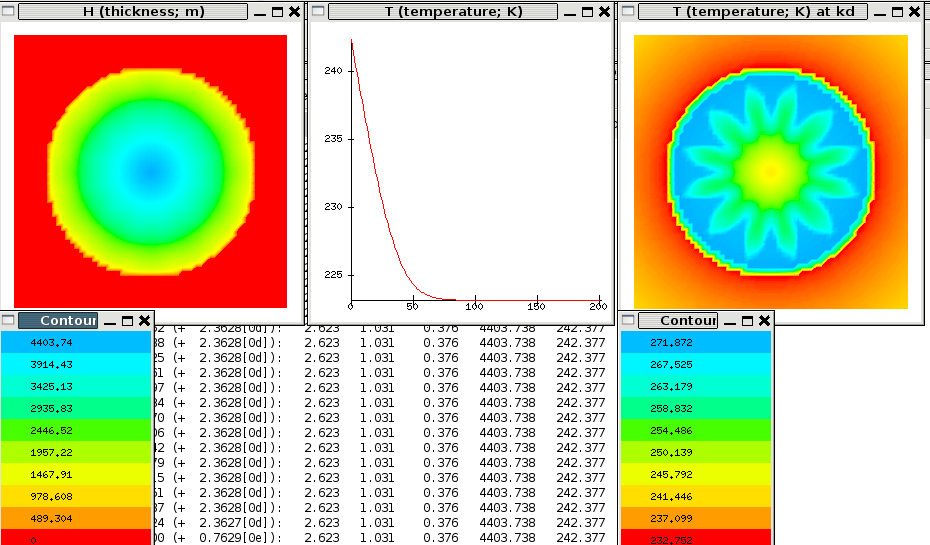
\includegraphics[height=4.0in,keepaspectratio=true]{eqns3Deps/eisIIFshot}
\caption{Diagnostic figures at the end of a 200,000 year EISMINT II experiment F run, showing the famous spokes.}
\label{fig:screenshot}
\end{figure}

At each time step we get a summary of the model state at the end of the step.  The format of the summary is
\scriptsize\begin{verbatim}
    $$$$$      YEAR (+    STEP[N$]):     VOL    AREA    MELTF     THICK0     TEMP0
\end{verbatim}
\normalsize
The first five columns are flags telling the user which quantities are being updated at each time step.  A dollar sign appears if the quantity does not update.  From the left the positions are: [\t{b\$}] for bed elevation, [\t{vV\$}] for velocity, [\t{g\$}] for grain size, [\t{t\$}] for temperature (and age), and [\t{f\$}] for surface elevation (i.e.~a step of the flow equation has occurred).  (Regarding velocity, a lower case ``\texttt{v}'' indicates that the 3D velocity field has been updated, e.g.~as needed for the advection of temperature, while uppercase ``\texttt{V}'' indicates that only the vertically-averaged velocity, and the associated diffusivity, has been updated.)

The time (``\t{YEAR}'') and time step (``\t{STEP}'') are in years.  In the above example runs the time step is 60 years because that is the default maximum time step.  A small whole number and a single character flag appear in square brackets after the time step, and these explain what part of the (somewhat elaborate) adaptive time-stepping scheme was used to determine the time step.  ``\t{m}'', in particular, means that the step was the maximum allowed.

The next three columns are the volume of the ice in $10^6 \,\text{km}^3$, the area covered by the ice in $10^6\,\text{km}^2$, and the basal melt fraction, that is, the fraction of the ice area where the basal homologous temperature is above $273.0$ (i.e.~slightly lower than the melting temperature).  The next two columns ``\texttt{THICK0}'' and ``\texttt{TEMP0}'' are values at the center of the computational domain, that is, the thickness at the origin in meters, and the basal absolute temperature at the origin in Kelvin.

This summary of the model state can be expanded by using the option \verb|-verbose|; an example of the result is discussed in the Verification section under ``Test I.''

For more on simplified geometry experiments, and standardized validations, see the Simplified Geometry and Validation section.

\subsection{Visualizing the results}  There are three modes for visualizing the various quantities in PISM.\begin{itemize}
\item At runtime various diagnostic viewers can be specified by options of the form \verb|-d HTt|; see the Usage and options section below.  These viewers are updated at each step and work under X windows.  The format is limited by the style of PETSc viewers, but in fact these viewers may suffice for many routine purposes.
\item The state of the model can be output in NetCDF format using the option \verb|-o foo -of n| to create the NetCDF file \verb|foo.nc|.  The resulting NetCDF file can be viewed with several available tools.
\item A \Matlab output file, in particular \Matlab script, can be produced by the options \verb|-o foo -of m|.  When executed in \Matlab, the script \verb|foo.m| records several two dimensional quantities, including two dimensional slices of three dimensional quantities.  The location of these slices is controlled by the options \verb|-id|, \verb|-jd|, \verb|-kd|.  See the Usage and options section below.
\end{itemize}


\subsection{Verification of PISM}  The purpose of the separate executable \t{pismv} is to establish that the code closely approximates an exact solution to the continuum equations of the model, and thus to check on the correctness of the code.  Thus \t{pismv} should be used when a new copy of PISM is installed, and especially when changes to the source code occur.

Also, one wants to understand the limits on \emph{reportable accuracy} from an ice sheet simulation, and the verification tests give some indication of this.  Of course the exact solutions have significantly simplified boundary conditions etc., and in some cases they are not very physical.

There are several types of exact solution based tests which verify several parts of the code, including the isothermal shallow ice approximation (SIA) \cite{BLKCB}, the thermomechanically coupled SIA \cite{BBL,BB}, sliding in the SIA \cite{BLKCB}, and the MacAyeal equations for ice streams as ``dragging ice shelves'' \cite{MacAyeal} with a plastic till assumption \cite{SchoofStream}.  The underlying ice model code executed by \t{pismv} is identical to that executed by \verb|run_ice|, but the command line options are somewhat different.

As noted in the Installation section, there is a script to execute a short selection of verifications, namely \t{pism/test/verifynow.sh}.  The standard results of that script appear in \t{pism/test/README.verifynow}.

Here is a basic isothermal verification example:

\beginV
user@host:~/pism$ obj/pismv -test B -ys 422.45 -ye 25000.0 -Mx 31 -My 31
\end{verbatim}
\Vend

Several behaviors were specified at the command line.  First, the code was \emph{run in parallel} under MPI (\texttt{www-unix.mcs.anl.gov/mpi/index.htm}) on two processors.  The exact solution Test B from \cite{BLKCB}, the Halfar solution \cite{Halfar83}, was used as the initial condition.  It is a zero accumulation isothermal solution and, instead of starting at a default time and specifying the number of years to run, here the starting and ending times as recommended in \cite{BLKCB} were given by options ``\t{-ys}'' and ``\t{-ye}''.  Note that as the sheet became thinner the adaptive time-stepping scheme lengthened the steps to the (default) maximum time step of 60 years.  A grid with $31\times 31$ points in the horizontal was used, matching the EISMINT 1996 choice \cite{EISMINT96} in the horizontal.  No diagnostic viewers were requested though they are available.

Errors at the final time are reported relative to the exact solution \cite{BLKCB}.  Note that the ``\t{-eo}'' flag can be given so that \t{verify} produces only the exact solution and does no numerics:
\beginV
    user@host:~/ice$ ./verify -test B -ys 422.45 -ye 25000.0 -Mx 31 -My 31 -eo
PISMV (verification mode)
  [using flow law 1 (where 0=Paterson-Budd,1=cold P-B,2=warm P-B,3=Hooke,4=Goldsby-Kohlstedt)]
initializing Test B ...
  [computational box for ice: ( 2400.00 km) x ( 2400.00 km) x ( 4000.00 m)]
  [grid cell dimensions     : (   80.00 km) x (   80.00 km) x (  133.33 m)]
running test B ...
$$$$      YEAR (+    STEP[N$]):     VOL    AREA MELTFabs     THICK0     TEMP0
$$$$    422.45 (+  0.0000[0 ]):   4.006   1.773    1.000   3600.000   283.454
$v$f    438.36 (+ 15.9085[0d]):   4.006   2.131   <same>   3587.401    <same>
$v$f    454.82 (+ 16.4574[0d]):   4.006   2.131   <same>   3574.205    <same>
$v$f    471.84 (+ 17.0201[0d]):   4.006   2.131   <same>   3560.570    <same>
$v$f    489.43 (+ 17.5941[0d]):   4.006   2.131   <same>   3546.692    <same>
\dots
$v$f   1793.45 (+ 56.0058[0d]):   4.006   2.464   <same>   3070.178    <same>
$v$f   1851.04 (+ 57.5971[0d]):   4.006   2.464   <same>   3059.478    <same>
$v$f   1910.27 (+ 59.2284[0d]):   4.006   2.464   <same>   3048.854    <same>
$v$f   1970.27 (+ 60.0000[0m]):   4.006   2.464   <same>   3038.460    <same>
$v$f   2030.27 (+ 60.0000[0m]):   4.006   2.464   <same>   3028.416    <same>
$v$f   2090.27 (+ 60.0000[0m]):   4.006   2.464   <same>   3018.700    <same>
\dots
$v$f  24770.27 (+ 60.0000[0m]):   4.006   3.130   <same>   2295.434    <same>
$v$f  24830.27 (+ 60.0000[0m]):   4.006   3.130   <same>   2294.816    <same>
$v$f  24890.27 (+ 60.0000[0m]):   4.006   3.130   <same>   2294.200    <same>
$v$f  24950.27 (+ 60.0000[0m]):   4.006   3.130   <same>   2293.586    <same>
$v$f  25000.00 (+ 49.7274[0e]):   4.006   3.130   <same>   2293.078    <same>
done with run
Actual ERRORS evaluated at final time (relative to exact solution):
geometry  :  prcntVOL  prcntAREA       maxH       avH   relmaxETA    domeH
               0.0053    11.8993   146.9380    8.2654    0.020601   5.3977
writing model state to file `verify.pb' ... done
\end{verbatim}
\Vend

Here we see the adapative time-stepping in action.  The exact solution being approximated here is the constant volume ice sheet which starts at time 0 as a delta function and spreads into a thinner and thinner ice sheet under the SIA \cite{BLKCB,Halfar83}.  At the end of this \t{pismv} verification run the errors are reported.  These are the differences between the values computed numerically on the grid and the known exact solution at the same grid points.  In particular, there are maximum thickness errors of up to 147 meters but the average thickness error is only 8.2 meters at the final time of 25,000 years (and on this very rough $31\times 31$ point grid).

An illuminating verification run for the thermomechanically coupled SIA is to use Test G from \cite{BBL}, and to watch the evolution of the sheet. [DESCRIBE TEST G AND ALSO TEST I]

[FORWARD REFERENCE TO Verification section] 


\section{Runtime options}

\newcommand{\opt}[1]{\vspace{1mm}\noindent \large\texttt{-#1}\,:\quad\normalsize}
\newcommand{\optdef}[2]{\vspace{1mm}\noindent \large\texttt{-#1}\,[\textsl{#2}]:\quad\normalsize}
\newcommand{\optrestrict}[2]{\vspace{1mm}\noindent \large\texttt{-#1}\,[\texttt{#2} \textsl{only}]:\quad\normalsize}
\newcommand{\optdefrestrict}[3]{\vspace{1mm}\noindent \large\texttt{-#1}\,[\textsl{#2}]\,[\texttt{#3} \textsl{only}]:\quad\normalsize}
\newcommand{\und}{$\underline{\,\,\,}$}

Much of the behavior of PISM can be set at the command line by options.  The format of the option, and the documentation below, is

\centerline{``\optdefrestrict{optionname}{A}{B} Description.''}

\noindent Here ``A'' is the default value and ``\t{B}'' is a list of the allowed executables.  The option applies to all executables (\verb|pismr|, \verb|pisms|, \verb|pismv|) unless the allowed executables are specifically stated by giving ``[\t{B} \textsl{only}]''.

As PISM is a PETSc program, all PETSc options are available \cite{petsc-web-page,petsc-user-ref}.  See the next subsection, which recalls some of these PETSc options.
\bigskip

\optdef{adapt\und ratio}{0.12}  Adaptive time stepping ratio for the explicit scheme for the mass balance equation.

\optrestrict{bal\und vel}{get\und drag}  

\opt{bed\und def\und iso} Compute bed deformations by simple pointwise isostasy.  Assumes that the bed at the starting time is in equilibrium with the load so the bed elevation is equal to the starting bed elevation minus a multiple of the increase in ice thickness from the starting time, roughly: $b(t,x,y) = b(0,x,y) - f [H(t,x,y) - H(0,x,y)]$.  Here $f$ is the density of ice divided by the density of the mantle.  See Test H in Verification section.

\opt{bed\und def\und lc} Compute bed deformations, caused by the changing load of the ice, using a viscoelastic earth model.  Uses the model and computational technique described in \cite{BLKfastearth}, based on the continuum model in \cite{LingleClark}.

\optrestrict{bif}{pismr}  The model can be ``bootstrapped'' from certain NetCDF files with just the right information.  Email \verb|ffelb@uaf.edu| for more info.  Compare \verb|-if|.

\optdef{constant\und nu}{30.0}  If this option is used then the MacAyeal velocities (see \verb|-mv| below) are computed with a constant viscosity.  If this option is not used then the viscosities are computed by a nonlinear iteration.  The argument is given in units of MPa a, and the default value is $30$ MPa a, the value given in \cite{Ritzetal2001}.

\opt{d}  Specifies diagnostic (X Windows) viewers.  See Diagnostic viewers section below.

\optdefrestrict{datprefix}{PISM}{pisms -ismip H}  Specify base name for ISMIP-HEINO deliverable \verb|.dat| files.  See also \verb|-no_deliver|.

\opt{dbig}  Specifies larger (about twice linear dimensions) diagnostic viewers.  See Diagnostic viewers section.

\opt{dx}  \emph{Use of this option is not recommended.}  \verb|dx| is computed internally as \verb|2*Lx/(Mx-1)|.  The user may alter \verb|Lx| or \verb|Mx| at the command line.

\opt{dy}  \emph{Use of this option is not recommended.}  \verb|dy| is computed internally as \verb|2*Ly/(My-1)|.  The user may alter \verb|Ly| or \verb|My| at the command line.

\opt{dz}  \emph{Use of this option is not recommended.}  \verb|dz| is computed internally as \verb|Lz/(Mz-1)|.  The user may alter \verb|Lz| or \verb|Mz| at the command line.

\optdef{e}{1.0}  Flow enhancement factor.

\optrestrict{eo}{pismv}  See Verification section.

\optdefrestrict{eisII}{A}{pisms}  Choose single character name of EISMINT II \cite{EISMINT00} simplified geometry experiment.  Allowed values are A, B, C, D, E, F, G, H.

\optrestrict{force\und quarter\und year}{pisms -ismip H}  ISMIP-HEINO specifies rigid $0.25$ year time steps.  This will violate both the diffusivity and the CFL parts of the adaptive time-stepping scheme.  This overrides the adaptime time-stepping and does $0.25$ year time steps anyway.

\optrestrict{gk}{pisms,pismr}  Sets the flow law to Goldsby-Kohlstedt.  Same as \verb|-law 4|.  See \verb|-law| for more complete option choice of flow law.]

\opt{history}  \emph{Use of this option is not recommended.}  It is usually desirable to keep the stored command history unaltered.

\optdef{id}{0}

\opt{if}  The model can be restarted from either a PETSc binary file written by the model, e.g.~\verb|foo.pb| from \verb|-o foo| or \verb|-o foo -of p|, or from a NetCDF file \verb|foo.nc| written by the model, e.g.~\verb|foo.nc| from \verb|-o foo -of n|.  Compare \verb|-bif|.

\optdefrestrict{ismip}{H}{pisms}  Choose ISMIP simplified geometry experiment.  Only ``H'' for HEINO is allowed at this time.

\opt{isoflux}  Isothermal runs can be done by two methods.  One may simply initialize with a constant temperature field and then turn off temperature evolution (see \verb|-no_temp|); in this case the horizontal velocity and the horizontal mass flux are computed by a vertical numerical integral.  If the option \verb|-isoflux| is used then the mass flux is computed by the usual isothermal, Glen formula without reference to the temperature field or the chosen flow law.

\optdef{jd}{0}

\optdef{kd}{0}

\begin{table}
\caption{Choosing the flow law.}\label{tab:flowlaw}
\begin{tabular}{@{}llll}\hline
\small
\textbf{Flow Law} & \textbf{Option} & \textbf{Comments and Reference} \\ \hline
Paterson-Budd law   &  \t{-law 0} &   Fixed Glen exponent $n=3$.  There is a split ``Arrhenius'' \\
  & & term $A(T) = A \exp(-Q/RT^*)$ where \\
  & & $(A = 3.615 \times 10^{-13}\, \text{s}^{-1}\, \text{Pa}^{-3}, Q = 6.0 \times 10^4\, \text{J}\, \text{mol}^{-1})$ if \\
  & & $T^* < 263$ K and $(A = 1.733 \times 10^{3}\, \text{s}^{-1}\, \text{Pa}^{-3}$, \\
  & & $Q = 13.9 \times 10^4\, \text{J}\, \text{mol}^{-1})$ if $T^* > 263$ K and \\
  & & where $T^*$ is the homologous temperature \cite{PatersonBudd}.  \\
\emph{Cold} part of Paterson-Budd    &  \t{-law 1} &   Regardless of temperature, the values for $T^*<263$ K in \\
  & & the Paterson-Budd law above apply.  This is the flow law \\
  & & used in the thermomechanically coupled exact solutions \\
  & & Tests \textbf{F} and \textbf{G} described in \cite{BBL,BB} \\
  & & and run by \verb|pismv -test F|,  \verb|pismv -test F|.  \\
\emph{Warm} part of Paterson-Budd     &  \t{-law 2} & Regardless of temperature, the values for $T^*>263$ K in \\
  & &  Paterson-Budd apply.    \\
Hooke law   &  \t{-law 3} &  Fixed Glen exponent $n=3$.  Here \\
  & & $A(T) = A \exp(-Q/(RT^*) + 3C (T_r - T^*)^\kappa)$; values of \\
  & & constants as in \cite{Hooke,PayneBaldwin}.   \\
Hybrid of Goldsby-Kohlstedt &  \t{-law 4} &     Goldsby-Kohlstedt law with a combination of exponents  \\
  \qquad and Paterson-Budd & & from $n=1.8$ to $n=4$ \cite{GoldsbyKohlstedt} in grounded \\
  & & shallow ice approximation regions.  Paterson-Budd flow \\
  & & for ice streams and ice sheets. See mask for SIA \\
  & & versus stream versus shelf by \verb|-d m|. \\
\hline
\normalsize
\end{tabular}
\end{table}

\optdef{law}{0}  Allows choice of thermocoupled flow law.  The options are in table \ref{tab:flowlaw} below.  Note that a ``flow law'' here means the function $F(\sigma,T,P,d)$ in the relation
	$$\dot \eps_{ij} = F(\sigma,T,P,d)\, \sigma_{ij}'$$
where $\dot \eps_{ij}$ is the strain rate tensor, $\sigma_{ij}'$ is the stress deviator tensor, $T$ is the ice temperature, $\sigma^2 = \frac{1}{2} \|\sigma_{ij}'\|_F$ so $\sigma$ is the second invariant of the stress deviator tensor, $P$ is the pressure, and $d$ is the grain size.  That is, we are addressing isotropic flow laws only, and one can choose the scalar function.  Note that the inverse form of such a flow law in needed for ice shelves and ice streams:
	$$\sigma_{ij}' = 2 \nu(\dot\eps,T,P,d)\,\dot \eps_{ij} $$
Here $\nu(\dot \eps,T,P,d)$ is the effective viscosity.  The need for this inverse form of the flow law explains the ``hybrid'' law \verb|-law 4| (or \verb|-gk|).


\opt{Lbz}  \emph{Use of this option is not recommended.}  The vertical thickness of the bed in which temperature is modeled is kept internally as the product \verb|Mbz*dz|.  The user may alter \verb|Mbz| at the command line.

\opt{Lx}

\opt{Ly}

\opt{Lz}

\optdef{maxdt}{60.0}

\optdef{Mbz}{0}

\optrestrict{Mmax}{pisms -eisII}  Set value of $M_{\text{max}}$ for EISMINT II.

\opt{mv}  Use the MacAyeal-Morland equations for ice shelves and dragging ice shelves (i.e.~ice streams) where so-indicated by the mask.  To view the mask use \verb|-d m|.

\optdef{mv\und eps}{1.0e15}  The numerical scheme for the MacAyeal-Morland equations computes an effective viscosity which which depends on velocity and temperature.  After that computation, this constant is added to the effective viscosity (to keep it bounded away from zero).  The units are kg $\text{m}^{-1}\,\text{s}^{-1}$.

\optdef{mv\und rtol}{1.0e-4}  The numerical scheme for the MacAyeal-Morland equations does a nonlinear iteration wherein velocities (and temperatures) are used to compute an effective viscosity which is used to solve the equations for velocity.  Then the new velocities are used to recompute an effective viscosity, and so on.  This option sets the relative change tolerance for the effective viscosity.

\optdef{Mx}{61}  Set number of grid points in horizontal direction.

\optdef{My}{61}  Set number of grid points in horizontal direction.

\optdef{Mz}{31}  Set number of grid points in vertical direction.

\optdef{mu\und sliding}{3.17e-11}

\opt{mv} Turn on solution of MacAyeal equations \cite{MacAyeal} in ice streams and ice shelves.
 
\optdef{mv\und eps}{}
 
\optdef{mv\und rtol}{}
 
\optrestrict{no\und deliver}{pisms -ismip H}  Do not write \verb|.dat| deliverable files in ISMIP-HEINO.

\opt{no\und mass}  Do not change surface elevations or thicknesses.  That is, do not do time steps of mass conservation equation.

\optrestrict{nreport}{pismv}  Do not report errors at the end of a verification run.

\optdef{no\und spokes}{0}  The strain heating term can be smoothed by non-physical averaging the neighboring horizontal neighbors (those which are within the ice) \cite{BBL}.  The integer parameter controls the number of neighboring grid points over which the average is computed.  For instance, \verb|-no_spokes 0| is no smoothing while \verb|-no_spokes 3| is smoothing over the 3-neighborhood of horizontal grid points, that is, over a distance of \verb|3*dx|.

\opt{no\und temp}  Do not change temperature or age values within the ice.  That is, do not do time steps of energy conservation and age equation.

\optdef{o}{unnamed.pb} Give name of output file: \verb|-o foo| writes an output file named \verb|foo.pb|.  See \verb|-if|; note model can be restarted from a PETSc binary file, e.g.~\verb|foo.pb|.  Default name is \verb|unnamed.pb| under \verb|pismr|, \verb|simp_exper.pb| under \verb|pisms|, and \verb|verify.pb| under \verb|pismv|.

\opt{ocean\und kill}  If used with input from a NetCDF initialization file which has ice-free ocean mask, will zero out ice thicknesses in areas that were ice-free ocean at time zero.  Has no effect when used with \verb|-no_mass|.

\optdef{of}{p}  Format of output file(s).  Possible values are \verb|p| for the model state written to a PETSc binary file, e.g.~\verb|foo.pb|, \verb|n| for model state written to a NetCDF file \verb|foo.nc|, and \verb|m| for selected variables written to an ASCII Matlab file \verb|foo.m|.  From resulting output \verb|.pb| and \verb|.nc| files, PISM can be restarted using \verb|-if|.  Compage \verb|-bif|.  By default an output file is written according to the name given by \verb|-o|.  Multiple files can be written, for instance, \verb|-o foo -of pm| writes both \verb|foo.pb| and \verb|foo.m|.

\opt{pause}    Pause for given number of seconds.  Allowed for \verb|pisms -ross| and \verb|pismv -test I|.

\optrestrict{prefix}{pisms -ross}    Set the data file prefix for the EISMINT Ross ice shelf validation \cite{MacAyealetal}.  See \verb|-ross|.

\optrestrict{plastic\und reg}{pismv -test I}    Set value of $\eps$ regularization of plastic till.  See \t{src/iceExactStreamModel.cc}.

\opt{regrid}

\opt{regrid\und vars}

\optrestrict{Rel}{pisms -eisII}    Set value of $R_{\text{el}}$ for EISMINT II.

\optrestrict{ross}{pisms}    Run the EISMINT Ross ice shelf validation \cite{MacAyealetal}.  Requires data from \url{http://homepages.vub.ac.be/~phuybrec/eismint/iceshelf.html}.

\optdefrestrict{run}{ST}{pisms -ismip H}  ISMIP-HEINO has several run names: ST, T1, T2, B1, B2, S1, S2, S3.

\optrestrict{Sb}{pisms -eisII}    Set value of $S_b$ for EISMINT II.

\optrestrict{showobsvel}{pisms -ross -d c}    Show the map of observed velocity for the EISMINT Ross ice shelf validation \cite{MacAyealetal}.  See \verb|-ross|.

\optrestrict{ST}{pisms -eisII}    Set value of $S_T$ for EISMINT II.

\optdef{tempskip}{1}  Number of mass-balance steps to perform before a temperature step is executed.  A maximum value of \verb|-tempskip 5| is recommended to avoid too many CFL violations.

\optdefrestrict{test}{A}{pismv}  Choose single character name of verification test.  Allowed values are A, B, C, D, E, F, G, H, I.  See the Verification section.

\optrestrict{time1}{pisms -ismip H}  ISMIP-HEINO requires writing 2D planform \verb|.dat| files at four times in the interval $[150,200]\times 10^{3}$ years.  This specifies the time.  Note \verb|test/showheino.m| will compute the time from the other \verb|.dat| files.

\optrestrict{time2}{pisms -ismip H}  See \verb|-time1| explanation.

\optrestrict{time3}{pisms -ismip H}  See \verb|-time1| explanation.

\optrestrict{time4}{pisms -ismip H}  See \verb|-time1| explanation.

\optrestrict{Tmin}{pisms -eisII}    Set value of $T_{\text{min}}$ for EISMINT II.

\optrestrict{tune}{pisms -ross}    Tune the vertically averaged hardness $\bar B$ in the EISMINT Ross ice shelf validation \cite{MacAyealetal}.  See \verb|-ross|.  A range of values can be given; see \verb|src/iceROSSModel.cc|.

\opt{verbose}   Increased verbosity of standard output.  Can be given without argument (``\verb|-verbose|'') or with a level which is one of the integers 0,1,2,3,4,5 (``\verb|-verbose 2|'').  The full scheme is given in table \ref{tab:verbosity}.

\begin{table}
\caption{Controlling the verbosity level to standard out.}\label{tab:verbosity}
\begin{tabular}{@{}llll}\hline
\small
\textbf{Level} & \textbf{Option} & \textbf{Meaning} \\ \hline
   0  &  \t{-verbose 0} &   never print to standard out \emph{at all}  \\
   1  &  \t{-verbose 1} &   less verbose than default  \\
   2  &  [\t{-verbose 2}] & default verbosity    \\
   3  &  \t{-verbose 3} &   somewhat verbose; expanded description of grid at start  \\
      &  or \quad \t{-verbose} &  and expanded information in summary    \\
   4  &  \t{-verbose 4} &     \\
      &  or \quad \t{-vverbose} &  more verbose    \\
   5  &  \t{-verbose 5} &     \\
      &  or \quad \t{-vvverbose} &  maximally verbose \\
\hline
\normalsize
\end{tabular}
\end{table}

\opt{vverbose}   See table \ref{tab:verbosity}.

\opt{vvverbose}   See table \ref{tab:verbosity}.

\optdef{y}{1000} Number of model years to run.

\opt{ye} Model year at which to end the run.

\opt{year}  Internally stored model year.  Modify this with some caution.  Certain non-physical runs (e.g.~under the executable \verb|pismv|) attach modeling meaning to the year.  That is, verification runs and others will \emph{not} be time-invariant.

\opt{ys} Model year at which to start the run.


\subsection{Additional options (for any PETSc program)}  All PETSc programs allow command line options which control the manner in which PETSc distributes jobs among parallel processors and how it solves linear systems (in particular).  The PETSc manual (\url{http://www.mcs.anl.gov/petsc/petsc-as/snapshots/petsc-current/docs/manual.pdf}) is the complete reference on these, but we list some that are of known importance to PISM users.

\opt{da\und processors\und x}

\opt{da\und processors\und y}  See \verb|-da_processors_x|.

\opt{help}

\opt{info}

\optdef{ksp\und rtol}{1e-5}

\optdef{ksp\und type}{gmres}  \t{bicg}, \t{cg}, \t{cgs}, \t{gmres}, \t{preonly}

\opt{log\und summary}

\optdef{pc\und type}{ilu}   \t{jacobi}, \t{icc}, \t{ilu}, \t{lu}, \t{none}, \t{sor}

\opt{v}   Show version number of Petsc.


\section{Diagnostic viewers} 

Many basic views of the changing state of the ice model are available at the command line by using the options ``\t{-d}'' and ``\t{-dbig}'' with additional arguments.  For instance:
\begin{verbatim}
   obj/pismr ... -d hTg -dbig c
\end{verbatim}
shows a map-plane views of surface elevation (``\t{h}''), temperature at the level specified by \t{-kd} (``\t{T}''), rate of change of thickness (``\t{g}'') and of vertically-averaged horizontal ice speed (``\t{c}'').

The option \t{-d} is followed by a space and then a list of single-character names of the diagnositic viewers.  The option \t{-dbig} works exactly the same way, with the same list of single-character names available.  The bigger viewers take precedence, so that ``\t{-d hT -dbig T}'' shows two viewers, namely a regular size viewer for surface elevation and a larger viewer for temperature.

The single character names are:

\verb|a|:\quad Map-plane view of accumulation in meters per year.

\verb|b|:\quad Map-plane view of bed elevation in meters above sea level.

\verb|c|:\quad Map-plane view of horizontal speed, namely the absolute value of the vertically-averaged horizontal velocity.  Displayed as log base ten of speed in meters per year.

\verb|D|:\quad Map-plane view of grain size, in millimeters.

\verb|d|:\quad Grain size in a vertical column (sounding); in millimeters.  See \verb|-id|, \verb|-jd| to set sounding location.

\verb|E|:\quad Map-plane view of age of the ice, in years.

\verb|d|:\quad Age in a vertical column (sounding); in years.  See \verb|-id|, \verb|-jd| to set sounding location.

\verb|f|:\quad Map-plane view of diffusivity coefficient $D$ in mass balance equation in $\text{m}^2/s$.  Meaningful only in regions of shallow ice flow.

\verb|G|:\quad Map-plane view of basal geothermal heat flux, in milliWatts per meter squared.

\verb|g|:\quad Map-plane view of rate of change in thickness in meters per year.

\verb|H|:\quad Map-plane view of thickness in meters.

\verb|h|:\quad Map-plane view of ice surface elevation in meters above sea level.

\verb|k|:\quad Iteration monitor for the Krylov subspace routines (KSP) in Petsc.  Shows norm of residual versus iteration number.

\verb|l|:\quad Map-plane view of basal melt rate in meters per year.

\verb|L|:\quad Map-plane view of basal melt water thickness in meters.

\verb|m|:\quad Map-plane view of mask for flow type:  \textbf{1} = grounded shallow ice sheet flow,  \textbf{2} = dragging ice shelf, \textbf{3} = floating ice shelf.

\verb|N|:\quad

\verb|n|:\quad

\verb|P|:\quad \emph{ONLY AVAILABLE for }\t{verify}.  Map-plane view of comPensatory heating term $\Sigma_C$ in thermocoupled verification tests F and G.  Displayed at chosen elevation above base; see option \verb|-kd|.

\verb|p|:\quad Map-plane view of bed uplift rate in meters per year.

\verb|q|:\quad Map-plane view of basal sliding speed.  Displayed as log base ten of speed in meters per year.

\verb|r|:\quad Map-plane view of surface temperature in Kelvin.

\verb|R|:\quad Map-plane view of basal frictional heating in milliWatts per meter squared.

\verb|S|:\quad Map-plane view of strain heating term $\Sigma$ in temperature equation, in Kelvin per year.  Displayed at chosen elevation above base; see option \verb|-kd|.

\verb|s|:\quad Strain heating term $\Sigma$ in vertical column (sounding).  See \verb|-id|, \verb|-jd| to set sounding location.

\verb|T|:\quad Map-plane view of basal temperature in Kelvin.

\verb|t|:\quad Temperature in vertical column (sounding).  See \verb|-id|, \verb|-jd| to set sounding location.

\verb|U|:\quad

\verb|u|:\quad

\verb|V|:\quad

\verb|v|:\quad

\verb|x|:\quad $x$-component of horizontal velocity in vertical column (sounding).  See \verb|-id|, \verb|-jd| to set sounding location.

\verb|X|:\quad Map plane view of x component of horizontal velocity, in meters per year.  Displayed at chosen elevation above base; see option \verb|-kd|.

\verb|y|:\quad $y$-component of horizontal velocity in vertical column (sounding).  See \verb|-id|, \verb|-jd| to set sounding location.

\verb|Y|:\quad Map plane view of y component of horizontal velocity, in meters per year.  Displayed at chosen elevation above base; see option \verb|-kd|.

\verb|z|:\quad Vertical velocity ($w$-component of velocity) in vertical column (sounding).  See \verb|-id|, \verb|-jd| to set sounding location.

\verb|Z|:\quad Map plane view of vertical velocity, in meters per year.  Displayed at chosen elevation above base; see option \verb|-kd|.


\subsection{Regridding}



\section{Verification}  ``Verification'' is a crucial task for a code as complicated as PISM.  It is a task not directly related to the physical behavior of real ice sheets, but rather it is exclusively mathematical and numerical.  It is the task of checking that the predictions of a numerical code, here PISM of course, are close to the predictions of the continuum model which the numerical code claims to approximate.  In particular, one compares exact solutions of the continuum model, if available, to their numerical approximations.

See \cite{BLKCB} and \cite{BBL} for discussion of verification issues for the isothermal and thermomechanically coupled shallow ice approximation (SIA), and for exact solutions to these models.  See \cite{BB} on the construction of solutions to the thermomechanically coupled SIA.  See \cite{SchoofStream} for an exact solution to the MacAyeal equations for ice streams using a plastic till assumption.

In PISM there is a separate executable \verb|pismv|, but the numerical code which is verified by \verb|pismv| is exactly the same sources as run by the executables \verb|pismr| and \verb|pisms|.  (In technical terms, \verb|pismv| runs a derived class of the core class \verb|IceModel|, which is most directly run by \verb|pismr|.)

Table \ref{tab:tests} summarizes the many exact solutions contained within PISM, and shows how to use them individually to verify and to measure accuracy.   Note that all of these exact solutions is a solution to a free boundary problem for partial differential equations.

\begin{table}
\caption{Exact solutions for verification in PISM.}\label{tab:tests}
\begin{tabular}{@{}llll}\hline
\small
\textbf{Test} & \textbf{Continuum model tested} & \textbf{Default invocation} & \textbf{Reference} \\ \hline
A & isothermal SIA (mass conservation) & \verb|pismv -test A -y 25000| & \cite{BLKCB} \\
B & isothermal SIA ('') & \verb|pismv -test B -ys 422.45 -y 25000| & \cite{BLKCB} \\
C & isothermal SIA ('') & \verb|pismv -test C -y 15208.0| & \cite{BLKCB} \\
D & isothermal SIA ('') & \verb|pismv -test D -y 25000| & \cite{BLKCB} \\
E & isothermal SIA ('' and sliding) & \verb|pismv -test E -y 25000| & \cite{BLKCB} \\
F & thermomechanically coupled SIA  & \verb|pismv -test F -y 25000| & \cite{BBL,BB} \\
 & \quad (mass conservation and energy) & & \\
G & thermomechanically coupled SIA ('') & \verb|pismv -test G -y 25000| & \cite{BBL,BB} \\
H & bed deformation coupled & \verb|pismv -test H -y 40034 -bed_def_iso| & \cite{BLKfastearth} \\
 & \quad with isothermal SIA & & \\
I & velocity computation using & \verb|pismv -test I -mv| & \cite{MacAyeal,SchoofStream} \\
 & \quad MacAyeal eqns and plastic till & & \\
\hline
\normalsize
\end{tabular}
\end{table}

For each of these tests, a serious attempt to verify requires going down a grid refinement path and measuring error.  For example, the runs
\beginV
obj/pismv -test B -ys 422.45 -y 25000 -Mx 31 -My 31 -Mz 11
obj/pismv -test B -ys 422.45 -y 25000 -Mx 61 -My 61 -Mz 11
obj/pismv -test B -ys 422.45 -y 25000 -Mx 121 -My 121 -Mz 11
obj/pismv -test B -ys 422.45 -y 25000 -Mx 241 -My 241 -Mz 11
\end{verbatim}
\Vend
will produce the error data which is displayed in figures 7, 8, 9, and 10 of \cite{BLKCB}.

For thermocoupled tests one would refine in three dimensions.  For example, the runs
\beginV
obj/pismv -test G -maxdt 10.0 -y 25000 -Mx 61 -My 61 -Mz 61
obj/pismv -test G -maxdt 10.0 -y 25000 -Mx 91 -My 91 -Mz 91
obj/pismv -test G -maxdt 10.0 -y 25000 -Mx 121 -My 121 -Mz 121
obj/pismv -test G -maxdt 10.0 -y 25000 -Mx 181 -My 181 -Mz 181
obj/pismv -test G -maxdt 10.0 -y 25000 -Mx 241 -My 241 -Mz 241
obj/pismv -test G -maxdt 10.0 -y 25000 -Mx 361 -My 361 -Mz 361
\end{verbatim}
\Vend
produce the error data in figures 13, 14, and 15 of \cite{BBL}.  (Don't do the last couple of these without a supercomputer!  The $361\times 361\times 361$ run involves more that $100$ million unknowns, updated at each of millions of time steps.)

Note there is a shell script, \verb|test/verifynow.sh|, which runs Tests C, G, and I, and suffices for basic verification of newly-installed copies of PISM.




\section{Simplified geometry}


\section{Validation}


\section{Realistic ice sheet modelling}


\section{Overview of the continuum model in PISM}
Significant features of the continuum model approximated by the PISM include:\begin{itemize}
\item The inland ice sheet is modeled with the thermocoupled shallow ice approximation equations \cite{Fowler}, and some temperature-activated basal sliding is allowed.
\item Ice shelves and ice streams are modeled by shallow equations which describe flow by longitudinal strain rates and basal sliding.  These equations are different from the shallow ice approximation.  In shelves and streams the velocities are independent of depth within the ice.  The equations were originally established for ice shelves \cite{Morland,MorlandZainuddin,MacAyealetal}.  They were adapted for ice streams, as ``dragging ice shelves,'' by \cite{MacAyeal}; see also \cite{HulbeMacAyeal}.
\item The regions of grounded ice in which the ice stream model is applied can be determined from mass balance velocities \cite{BamberVaughanJoughin} or from observed surface velocities.
\item A three dimensional age field is computed.
\item A temperature model for the bedrock under an ice sheet is included.
\item Geothermal flux which varies in the map-plane can be used, for instance based on the new Antarctic results in \cite{ShapiroRitzwoller} and \cite{FoxMaule}.
\item Within the shallow ice sheet regions the model can use the constitutive relation of Goldsby and Kohlstedt \cite{GoldsbyKohlstedt,Peltieretal}.  For inclusion in this flow law, grain size can be computed using a age-grain size relation from the Vostok core data \cite{VostokCore}, for example.
\item The \cite{LingleClark} bed deformation model can be used.  It combines a spherical elastic earth and viscous half-space asthenosphere/mantle.  This model can be initialized by an observed bed uplift map \cite{BLKfastearth}, or even an uplift map computed by an external model.\end{itemize}

Many of the parts of the model described above are optional.  For instance, the Paterson-Budd-Glen \cite{PatersonBudd} flow can replace the Goldsby-Kohlstedt law, a simple isostasy model can be substituted for the more sophisticated one, and so on.  Options can be chosen at the command line  as described in the Run-time options section above.

The following features are \emph{not} included in the continuum model, and would (or will) require major additions:
\begin{itemize}
\item Inclusion of all components of the stress tensor (i.e.~longitudinal stresses within the shallow ice approximation region and additional shear stress components in shelves/streams) through either an intermediate order scheme \cite{Blatter,SaitoEISMINT} or the full Stokes equations \cite{Fowler}.
\item A model for water--content within the ice.  In the current model the ice is \emph{cold} and not \emph{polythermal}; compare \cite{Greve}.  On the other hand, in the current model the energy used to melt the ice within a given column, if any, is conserved.  In particular, a layer of basal melt water evolves by conservation of energy in the column.  This layer can activate basal sliding and its latent heat energy is available for refreezing.
\item A model for basal water mass conservation in the map-plane; compare \cite{JohnsonFastook}.
\item A fully spherical Earth deformation model, for example one descended from the Earth model of \cite{Peltier}.
\end{itemize}

\section{Overview of the numerical schemes in PISM}
Significant features of the numerical method described in these notes and implemented in PISM, include:\begin{itemize}
\item Verification \cite{Roache} is a primary concern and is built into the code.  Nontrivial verifications are available for isothermal ice sheet flow \cite{BLKCB}, thermocoupled sheet flow \cite{BB,BBL}, the earth deformation model \cite{BLKfastearth}, the coupled (ice flow)/(earth deformation) system in an isothermal and pointwise isostasy  case \cite{BLKfastearth}, and the MacAyeal equations for ice stream flow \cite{SchoofStream,BrownPresentation}.
\item The code is \emph{structurally} parallel.  In fact, the PETSc toolkit is used at all levels \cite{petsc-web-page,petsc-user-ref}.  PETSc manages the MPI-based communication between processors, and provides an interface to parallel numerical linear algebra and other numerical functions.
\item The grid can be chosen at the command line.  Regridding can be done at any time, for example taking the result of a rough grid computation and interpolating it onto a finer grid.
\item A moving boundary technique is used for the temperature equation which does not stretch the vertical in a singular manner; the Jenssen \cite{Jenssen} change of variables is not used.
\item The model uses an explicit time stepping method for flow and a partly implicit method for temperature.  Advection of temperature is upwinded \cite{MortonMayers}.  As described  in  \cite{BBL}, reasonably rigorous stability criteria are applied to the time-stepping scheme, including the diffusivity-based criteria for the explicit mass continuity scheme and the CFL criteria \cite{MortonMayers} for temperature advection.  The local truncation error is $O(\Delta x,\Delta y,\Delta z,\Delta t)$.
\item MacAyeal equations \cite{MacAyeal,SchoofStream} are used to determine velocity in the ice shelf and ice stream regions, and they are nonlinear and nonlocal equations for the velocity given the geometry of the streams and shelves and the ice temperature.  They are solved by straightforward iteration of linearized equations with numerically-determined (vertically-averaged) viscosity.  Either plastic till or linear drag is allowed.  As with all of PISM, the numerical approximation is finite difference.  The linearized finite difference equations are solved by any of the Krylov subspace methods in PETSc \cite{BrownPresentation,petsc-web-page,petsc-user-ref}.
\item The bed deformation model is implemented by a new Fourier collocation (spectral) method \cite{BLKfastearth}.
\item Implementation is in C++ and is object-oriented.  For example, verification occurs in a derived class.
\end{itemize}


\section{User's overview of the PISM source code}  This ice sheet model is implemented as a collection of C++ object classes [REFERENCE], the most central of which is \t{IceModel}.

More elementary than \t{IceModel} are the classes\begin{itemize}
\item \t{IceGrid}, which describes the shape of the grid and parallel
layout. This abstraction could be used to streamline transferring model data between
different grids.
\item \t{MaterialType}.  Various materials are derived from the class \t{MaterialType} which merely defines a couple
physical constants. \t{IceType} is still an abstract class which defines the interface to
ice flow. Concrete classes derived from \t{IceType} are \t{ThermoGlenIce} (which uses the
EISMINT constants) and \t{GKIce} as well as \t{HybridIce}.  Similarly, there is \t{BedrockType} and \t{OceanType} which merely define
associated physical constants.\end{itemize}

An example derived class of \t{IceType} is \t{HybridIce}, as mentioned.  Note that it is difficult, at least, to implement a complete Goldsby-Kohlstedt ice type \cite{GoldsbyKohlstedt} since the inverse constitutive
relation is required for computation of MacAyeal-type ice shelf and dragging ice shelf \cite{MacAyeal} velocity fields. \t{HybridIce} is Goldsby-Kohlstedt ice in the interior of the ice sheet and Glen ice in ice streams and
shelves.

The methods for \t{IceModel} are many.  They initialize the model (from input data files or from formulas describing various exact solutions), they read user options, they allocate arrays in a distributed manner under PETSc, they compute the terms in the various continuum equations (mass balance, conservation of energy, and velocity), they control diagnostic viewers, they run the central time-stepping, and they write out the model state to files.

A derived class of \t{IceModel} called \t{IceCompModel} is used for verification; see the next section.  It has additional structures which allows \t{IceModel} to have compensatory sources and compute initial conditions from, and especially to report errors relative to, known exact solutions \cite{BLKCB,BBL,BB,SchoofStream}.

There are two established drivers which call constructors and destructors for \t{IceModel}, namely \verb|run_ice| and \verb|verify|; examples appear above.  These drivers include no computation but differ in which class is constructed (\t{IceModel} vs \t{IceCompModel}) and in how certain options are handled.  They invoke the same numerical proceedures to handle the various partial differential equations of the continuum model, and this fact, along with the derived class relation for \t{IceCompModel}, is at the heart of the verification mechanism.  Driver \verb|run_ice| should be used for actual ice sheet computations, based on data files which will typically be in NetCDF form.  Driver \verb|run_ice| should also be used for simulations of symmetrical or artificial sheets for which no exact solution is known (and, obviously, for which no compensatory sources are needed) such as the EISMINT experiments \cite{EISMINT96,EISMINT00}.  Driver \verb|verify| is simply for verification and reports errors relative to exact solutions.

\subsection{PETSc: An overview for PISM users}  The PETSc library \cite{petsc-web-page,petsc-user-ref,petsc-efficient} provides essential support for distributed arrays and linear solvers in a parallel computing environment.  ``PETSc'' stands for ``Portable, Extensible Toolkit for Scientific Computation.''  Specifically,it is a suite of data structures and routines in the C language, primarily, for the scalable (parallel) solution of scientific applications modeled by partial differential equations.  Large parts of PETSc relate especially to finite-difference type regular, rectangular grids.

Documentation for PETSc is available from the web site at \url{http://www-unix.mcs.anl.gov/petsc/petsc-as/}.

PETSc employs the MPI standard for all message-passing communication.  See the next section.

Most variables in a PETSc program are of newly-defined distributed types including
\begin{verbatim}
DA   da;
Vec  v;
KSP  ksp;
\end{verbatim}
In fact most of the PETSc types merely declare pointers but they should be regarded as objects (abstract data types).  The objects must be created with calls to functions like \t{DACreate2d()}, \t{VecCreate()}, etc.  They should be destroyed when they are not needed with calls to corresponding \t{Destroy()} functions.

\subsection{Distributed arrays and vectors}
PETSc has an abstract date type called a distributed array. Objects of type DA contain
information about the grid and stencil. They can have information about coordinates, but
the code does not use this feature at present. Vectors are created with
\texttt{DAVecCreate()} and similar. These vectors will be distributed across the
processors as indicated by the distributed array.

There are two parameters of note: stencil type and stencil width. The stencil types are
\verb|DA_STENCIL_STAR| and \verb|DA_STENCIL_BOX|. They are generalizations of the five
point and nine point stencils typical of two dimensional discretizations respectively. In
particular, \verb|DA_STENCIL_STAR| indicates that ghosted points (information owned by a
different processor) will be needed only along the coordinate axes while
\verb|DA_STENCIL_BOX| indicates that ghosted points will be needed in the box shaped
region surrounding each point. The stencil width indicates how many points in each
direction will be needed. We never need a stencil width greater than 1 and only need box
style stencils when gradient terms must be evaluated on a staggered grid ($h$ in SIA
velocity and $\bar{u},\bar{v}$ in computation of effective viscosity in Macayeal
velocity). We could keeping all other two dimensional vectors on a start type stencil
would reduce the necessary communication slightly, but would complicate the code. For this
reason, all two dimensional vectors are kept on a box type distributed array.

The three dimensional distributed arrays are aligned so that they have the same horizontal
extent as the associated two dimensional distributed array, but have complete vertical
extent. One point of confusion is the redefinition of the $x,y,z$ axes. Contrary to the
PETSc defaut, our $z$ axis changes most rapidly through memory while the $x$ axis changes
most slowly. That is, our C style arrays will be addressed as \texttt{u[i][j][k]} where
$\texttt{i,j,k}$ are the coordinate indices in the directions $x,y,z$ respectively. DA
based vectors can be accessed by \texttt{DAVecGetArray()} and restored with
\texttt{DAVecRestoreArray()}. The resulting pointer should be addressed using normal
multidimensional array indexing where values range over the global array.

PETSc DA based vectors can be ``local'' or ``global''. Local vectors include space for the
ghosted points. That is, when \texttt{DAVecGetArray()} is called, the resulting array can
be indexed on all the ghosted points. However, all vector operations act only on the local
portion. \texttt{DALocalToLocalBegin()} and then \texttt{DALocalToLocalEnd()} should be
called to update the ghost points before they will be needed. Global vectors do not hold
ghosted values, but array operations will act on the entire vector. Hence local vectors
typically need to be mapped to global vectors before viewing or using in a linear system.
This is achieved with \texttt{DALocalToGlobal()}.

\subsection{Solving linear systems}
PETSc is designed for solving large, sparse systems in a distributed environment.
Iterative methods are the name of the game and especially Krylov subspace methods such as
conjugate gradients and GMRES. For consistency, all methods use the Krylov subspace
interface. For this, the user declares an object of type \texttt{KSP}. Various options can
be set and the preconditioner context can be extracted. PETSc has an options database
which holds command line options. To allow these options to influence the \t{KSP}, one
should call \t{KSPSetFromOptions()} prior to solving the system. The default method is
GMRES(30) with ILU preconditioning.

To solve the system, a matrix must be attached to the \t{KSP}. The first time
\t{KSPSolve()} is called, the matrix will be factored by the preconditioner and reused
when the system is called for additional right hand sides. The default matrix format is
similar to the Matlab \t{sparse} format. Each processor owns a range of rows. Elements in
matrices and vectors can be set using \t{MatSetValues()} and \t{VecSetValues()}. These
routines use the global indexing and can set values on any processor. The values are
cached until one calls \t{MatAssemblyBegin()} followed by \t{MatAssemblyEnd()} to
communicate the values.

In the Macayeal velocity computation, the solution and right hand side vectors are not DA
based. The vector (field) components are interlaced and distributed. This seemed to be the
most straightforward method to solve the system (as opposed to using more advanced
features intended for multiple degrees of freedom on DA based vectors). This also allows
the matrix to have an optimal parallel layout.

\subsection{PETSc utility functions}
The \t{PetscViewer} interface allows PETSc objects to be displayed. This can be in binary
to disk, in plain text to the terminal, in graphical form to an X server, to a running
instance of Matlab, etc. Typically, one will want to view an entire vector, not just the
local portion, so DA based local vectors are mapped to global vectors before viewing. When
viewing multiprocessor jobs, the display may have to be set on the command line (ie.
\t{-display :0} or similar).

PETSc allows the programmer to access command line arguments at any time during program
execution. This is preferable to using \t{getopt.h} for this purpose. A convenient feature
is the \t{PetscBag} which is a serializable (can be written to disk) structure with
default values which can be set on the command line. A \t{PetscBag} is used for describing
the size of the grid. It is the first piece of data written to model state files so that
the program can start from the same state. Other options such as enhancement factors, ice
types and whether or not to use Macayeal velocity is not stored in a \t{PetscBag} at this
time.

Quite ellaborate error tracing and performance monitoring is possible with PETSc. All
functions return \t{PetscErrorCode} which should be checked by the macro \t{CHKERRQ()}.
Normally, runtime errors print traceback information when the program exits. If this
information is not present, you may need to use a debugger which is accessible with the
command line options \verb|-start_in_debugger| and \verb|-on_error_attach_debugger|. Also
consider options such as \verb|-log_summary| to get diagnostics written to the terminal.

\subsection{MPI}  MPI is a library which manages interprocessor communication for parallel computers.  One of the advantages of Petsc is that it calls MPI in a way that allows Petsc-using programs to be largely free of parallel communication details.


%         References
\bibliography{ice_bib}
\bibliographystyle{siam}


\end{document}
